
{\color{blue}4-26}

We will discuss
\begin{enumerate}
\item
Phase diagrams
\item
Critical behavior
\item
Scaling limits
\end{enumerate}

\section{Phase diagrams}

\begin{theorem}
For any system of Ising spins on $\mathbb{Z}^d$ with a finite range, translation-invariant interactions of the form
\be
H=H_0 - h\sum_x \sigma_x,\qquad H_0(\sigma) = -\sum_A J_A\sigma_A, \qquad \sigma_A=\prod_{x\in A}\sigma_x
\ee
there is $T_0$ such that for all $T>T_0$ (equivalently $\beta<\beta_0$) there is a unique infinite-volume Gibbs state $\mu_{\beta, h}$ such that
\begin{enumerate}
\item
For any local $F\in \mathcal{B}_0$, $\mu_{\beta,h}(F)$ is analytic in $\beta$ and in the interaction parameter.
\item
$\frac{\partial}{\partial J_B} \left\langle {\sigma_B}\right\rangle = \left\langle {\sigma_A\sigma_B}\right\rangle - \left\langle {\sigma_A}\right\rangle\left\langle {\sigma_B}\right\rangle :=\left\langle {\sigma_A;\sigma_B}\right\rangle$.
\item
(Strength of correlation decays exponentially.) $|\left\langle {\sigma_A;\sigma_B}\right\rangle|\le Ce^{-d(A,B)}$ for some $C$.
\end{enumerate}
Furthermore for each $T>0$, (1)--(3) hold for all $|h|$ large enough.
\end{theorem}

Note infinite temperature gives the product measure, and the properties hold trivially. The theorem says the properties continue to hold for high enough temperature.

The theorem holds for models more general than Ising models; it holds in any system where spins take a finite number of values.

%$e^{-\be H_0}$
%dilute gas of particles. 
%There is a regime which can be cluster expansions and robust analysis, high magnetic field. Voting against field is excitation. Very dilute. Gibbs state depends on coupling. Analytically there are no phase transitions. 
%(2) true in finite volume. Further truncated... 

The proof is based on the technique of \index{cluster expansion}\textbf{cluster expansion}, and the earlier technique of Meyer expansion. A beautiful general technique was developed by Dobrushin %D of DLR
and Shlosman.\footnote{Like in Tolstoy's Anna Karenina, happy families are Gibbs states at high temperature; they are all alike.}
%Tolstoy, Anna Karenina.
%happy families are Gibbs states at high temperature; the are all alike

\begin{theorem}[Lee-Yang]
For the Ising model with $H=-\frac{1}{2} \sum_{x,y} J_{x,y} \sigma_x\sigma_y, J_{x,y} \ge 0$ ferromagnetic, at any $(T,h)$ with $T\ge 0$, $h\ne 0$, the Gibbs state is unique and analytic in $h$. %dreams of Riemann hypothesis.
%finite value partition can only have zeros along imaginary line.
\end{theorem}
The Gibbs state is analytic in $h$. The function may fail (and does fail) to be analytic along $h=0$ but nowhere else. 

The theorem is proven by establishing $Z_\Lambda (\beta, h)\ne 0$ for all $h\in \mathbb{C}\backslash \{\mathbb{R}\}$, $\Im h\ne 0$ for any finite graph.
%gibbs state as analytic in $h$.

A lesson from complex analysis is that convergence of power series along the real line are affected by singularities in the complex plane. They showed that singularities are purely along the imaginary line.

When the singularities approach 0, you get a function that has continuous singularities in the limit. As long as this does not happen, you have convergent power series in the magnetic field.

The technique includes beautiful complex analysis, but is very specific.

By the Peierls argument, there exists $T_p$ such that for $T<T_P$ such that for $T<T_P$ the magnetization is discontinuous in $h$,
\be
\lim_{h\searrow0\text{ (or }
h\nearrow0)}
\lim_{L\nearrow \infty} \left\langle {\sigma_0}\right\rangle_{\beta, h}^{\text{p.b.c}}
\left\langle {\sigma_0}\right\rangle_{\beta, 0+} = -\left\langle {\sigma_0}\right\rangle_{\beta, 0-} = m(\beta)>0.
\ee
Recall $\left\langle {\sigma_0}\right\rangle = \frac{1}{\beta} \frac{\partial}{\partial \beta}\Psi(\beta, h)$.
The order of limits is important. We take the infinite volume limit first.
%take infinite volume limit, obtain a state which we denote by $\an{-}_{\be, h}$, then take $\be\searrow 0$ or $\be \nearrow 0$.

%in any finite volume, is analytic in $h$.

In the early days of statistical mechanics this caused significant discussion. If you take the infinite volume limit first, you can develp all kinds of singularities.

At the cricial point, there's no discontinuity but the function has divergent slope. 

\begin{center}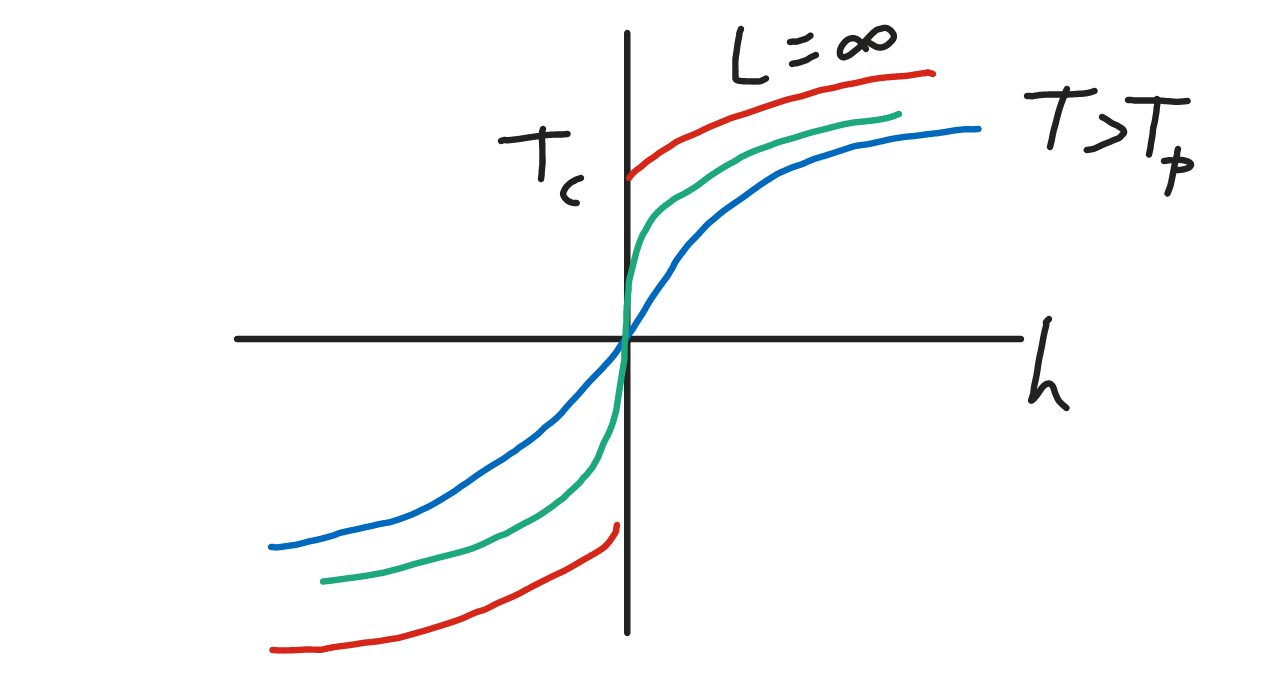
\includegraphics[scale=.25]{images/4-26-2}\end{center}

\begin{theorem}
For any ferromagnetic Ising model on $\mathbb{Z}^d$ with $0 \le J_{x-y} \le Ae^{-\frac{|x-y|}{\xi_0}}$, there exists $T_c<\infty$ such that 
\begin{enumerate}
\item
For all $T>T_c$, $m(T)=0$, $\left\langle {\sigma_x\sigma_y}\right\rangle\le \widetilde{A} e^{-\frac{|x-y|}{\xi}}$
\item
For all $T<T_c$, $m(T)>0$. 
\item
\begin{enumerate}
\item
At $h=0$, $T\searrow T_c$, the \index{magnetic susceptibility}\textbf{magnetic susceptibility} $\chi(T,0)\ge \frac{c}{|T-T_C|}$ where 
\begin{align}
\chi(\beta,h) &= \frac{\partial}{\partial h} \left\langle {\sigma_0}\right\rangle_{\beta, h} \\
&=\frac{1}{\beta}\frac{\partial^2 }{\partial {h}^2}\Psi(\beta, h)\\
&=\sum_x \left\langle {\sigma_0;\sigma_x}\right\rangle
\end{align}
(The {magnetic susceptibility} blows up at the critical temperature.)
\item
For $h=0$, $T\nearrow T_c$, $m(T) \ge c(T_c-T)^{\frac{1}{2}}$.
\item
For $T=T_c$, $h\searrow 0$, $m(T_c,h) \ge ch^{\frac{1}{3}}$.
\end{enumerate}
\end{enumerate}
Furthermore, for finite range models in $d>4$ dimensions these bounds also hold in the reverse directions (with different constants).
\end{theorem}
Much of this is true in 4 dimensions up to logarithmic constants.

In fact, it is true/conjectured that %(this is much harder to prove),
\begin{align}
\chi(T,0) &\sim \frac{c}{|T-T_C|^{\gamma}}, &\gamma &\ge 1\\
m(T) &\sim c(T_c-T)^{\frac{1}{\widehat{\beta}}},&\widehat{\beta} &\le 2\\
m(T_C)&\sim ch^{\frac{1}{\delta}}, &\delta&\ge 3.
\end{align}
%geometry of path expansions

The lace expansion technique is analogue of reflection positivity for finite range models.
%high  dimension is Gaussian.

The critical exponents are expected to be ``universal".
%independent of 
It's constant in a class of models which are categorized as being in the same class.

%only in a layer. Lower dimension. 
%Ferromagnetic, finite range. The critical points can change but... the same. 
%Do depend on the dimension. 

In 1 dimension there is no phase technology. In 2-D we know a lot, like explicit formulas. 3-D is of obvious physical interest and the results are hardest to come by.

For $d>4=:d_{\text{u.c.}}$ (the upper critical dimension),
\be
\gamma = \lim_{T\searrow T_c} \frac{\ln \chi(T,0)}{|T-T_c|^{-1}}
\ee
exists, etc., and the cricial exponents take their \textbf{mean-field values}.

\section{Mean-field theory}
There is an important lesson to take from here. Where the critical theory  is complicated, eventually in higher dimension it simplifies. A spectacular manifestation is that simple approaches produce correct results for the critical exponents.

Simplify the lattice by thinking of trees.

Take $\{\sigma_j\}_{j=1,\ldots, N}$, let 
\begin{align}
H &=-\frac{J}{2} \frac{1}{N} \sum_{x,y=1}^{N} \sigma_x\sigma_y - h\sum\sigma_x\\
& = -N\left[ {\frac{J}{2} M^2 + hM} \right], &M&=\frac{1}{N}\sum_{x=1}^{N} \sigma_x.
\end{align}
%want the force on each spin due to neighbors to be the same
This has just one degree of freedom, the bulk magnetization.

%over spin configurations.
Then
\begin{align}
\Psi(\beta, h)&=\lim_{N\to \infty} \log\left( {\sum_{\sigma_\Lambda = \pm1} e^{-\beta H_N(\sigma)}} \right)\\
&= \lim_{N\to \infty} \frac{1}{N} \log \sum_M e^{S(M)+\beta \frac{J}{2}M^2 + \beta h M}\\
%somewhere this is maximized, close values of $M$ are similar. $\ep$-different value is suppressed.
%by large deviation story
&=\sup_M [S(M) + \frac{\beta J}{2}M^2 + \beta hM].
\end{align}
Recall that the entropy is 
%M is average of $\pm$ spins.
%log of number of configuraitons.
\begin{align}
S(M) &= -\left[ {\left( {\frac{1+M}{2}} \right) \ln \left( {\frac{1+M}{2}} \right) + \left( {1-M} \right){2}\ln \left( {\frac{1-M}{2}} \right)} \right]\\
&=\ln 2 - \frac{1}{M}^2  - \frac{1}{12}M^4 + O(M^6).
\end{align}

For $h=0$, we have the following picture. 
%inverted parabolic behavior.
%pic

\begin{center}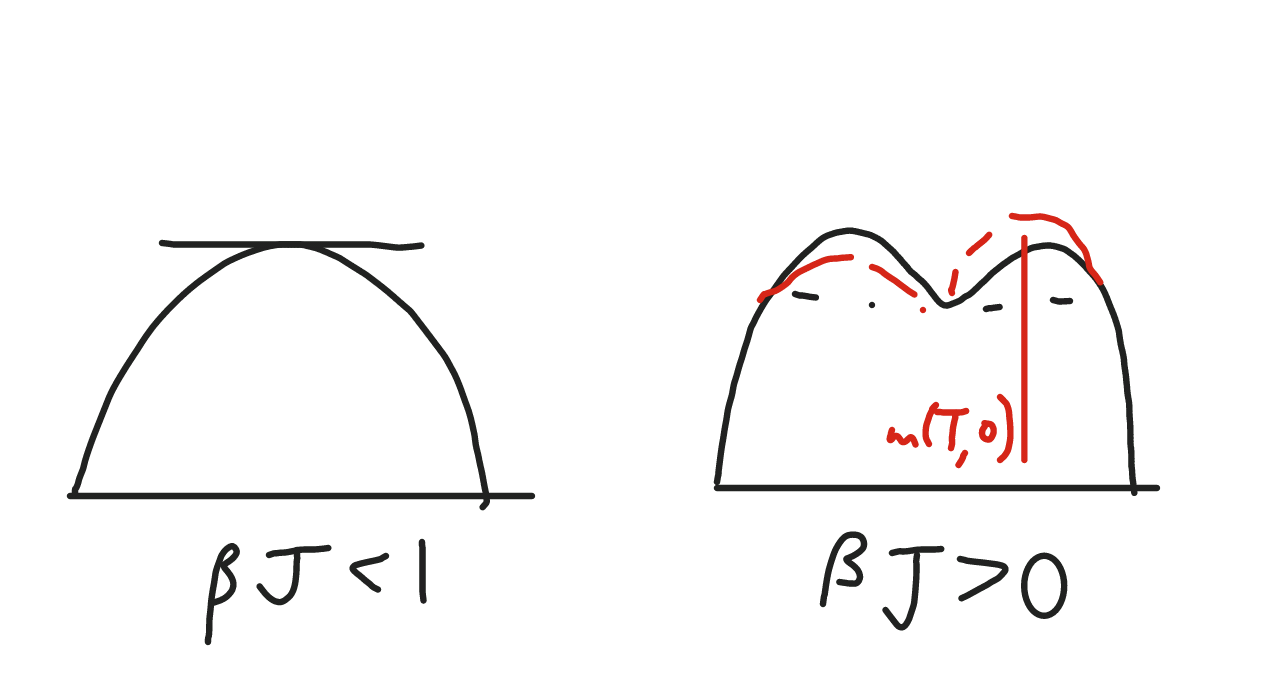
\includegraphics[scale=.25]{images/4-26-4}\end{center}


For $\beta J>1$, $\operatorname{argmax}(S(m) +\cdots)$ is discontinuous in $h$ at $h=0$.

%m(T,h)
We have $m(\beta,h)= \frac{1}{\beta} \frac{\partial}{\partial h}\Psi(\beta, h)$, 
\be
m(\beta, h) = \tanh(\beta J m + \beta h).
\ee
Where did we get this equation come from? This is the self-consistency equation. 

First consider the conditional magnetization. If everything interacts with each other, we get $\sigma_x(J\frac{1}{N} \sum \sigma_y + h)$ where $M=\frac{1}{N} \sum \sigma_y$. %under effect of magnetic field.

There are 3 solutions.

\begin{center}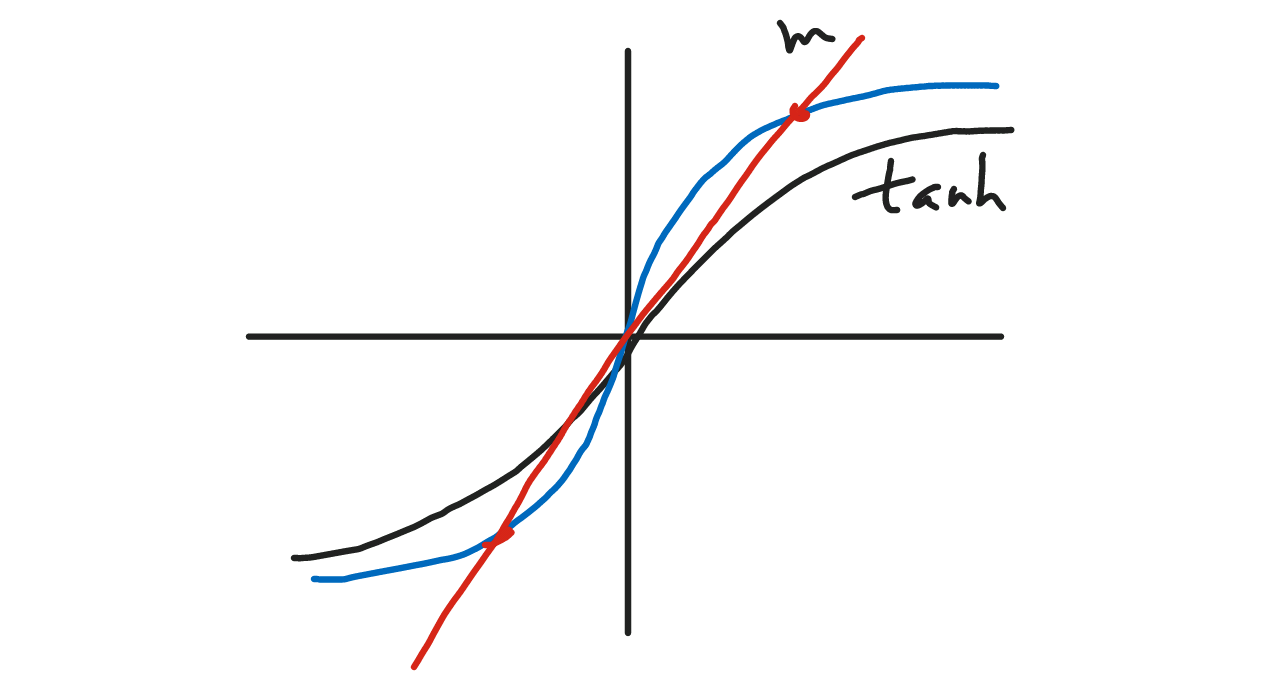
\includegraphics[scale=.25]{images/4-26-5}\end{center}

%value of total... doesn't fluctuate very much.
%hyperbolic tangent...
We can say the same for a finite system, except the magnetization from the neighbors fluctuates. In our setting, no single spin has much of an effect ($\frac{1}{N}$). 
